\documentclass[12pt,a4paper]{article}
\usepackage[utf8]{inputenc}
\usepackage[T1]{fontenc}
\usepackage[croatian]{babel}
\usepackage{lmodern}
\usepackage{microtype}
\usepackage{amssymb}
\usepackage{geometry}
\usepackage{graphicx}
\usepackage{listings}
\usepackage{xcolor}
\usepackage{hyperref}
\usepackage{tikz}
\usepackage{float}
\usepackage{tabularx}
\usepackage{booktabs}
\usepackage[most]{tcolorbox}
\usepackage{titlesec}
\usepackage{enumitem}
\usepackage{parskip}
\usetikzlibrary{positioning, arrows.meta, shapes.multipart, fit, calc, decorations.markings, backgrounds}

% ---- Deployment node 3D effect (UML deployment node look) ----
\newcommand{\deploybox}[2]{%
  \begin{scope}[on background layer]
    \draw[thick, fill=#2]
      (#1.north west) -- ++(0.22,0.28)
      -- ([shift={(0.22,0.28)}]#1.north east)
      -- (#1.north east) -- cycle;
    \draw[thick, fill=#2]
      (#1.north east) -- ++(0.22,0.28)
      -- ([shift={(0.22,0.28)}]#1.south east)
      -- (#1.south east) -- cycle;
  \end{scope}%
}

\geometry{margin=2.5cm}

% ---- Colors ----
\definecolor{codebg}{HTML}{F7F8FA}
\definecolor{codeframe}{HTML}{D0D7DE}
\definecolor{keyword}{HTML}{0550AE}
\definecolor{string}{HTML}{116329}
\definecolor{comment}{HTML}{6E7781}
\definecolor{accent}{HTML}{1F4E79}
\definecolor{accentlight}{HTML}{DCE6F1}
\definecolor{infoborder}{HTML}{2E86AB}
\definecolor{infobg}{HTML}{EAF3FA}

% ---- Section headers ----
\titleformat{\section}
  {\Large\bfseries\color{accent}}
  {\thesection}{0.7em}{}
  [\vspace{-0.3em}{\color{accent}\titlerule[1pt]}]
\titleformat{\subsection}
  {\large\bfseries\color{accent!85!black}}
  {\thesubsection}{0.6em}{}
\titlespacing*{\section}{0pt}{1.8em}{0.9em}
\titlespacing*{\subsection}{0pt}{1.2em}{0.5em}

% ---- Paragraph spacing ----
\setlength{\parskip}{0.6em}
\setlength{\parindent}{0pt}

% ---- Code listings ----
\lstset{
  basicstyle=\ttfamily\footnotesize,
  backgroundcolor=\color{codebg},
  frame=single,
  framesep=6pt,
  rulecolor=\color{codeframe},
  breaklines=true,
  columns=fullflexible,
  keywordstyle=\color{keyword}\bfseries,
  stringstyle=\color{string},
  commentstyle=\color{comment}\itshape,
  showstringspaces=false,
  captionpos=b,
  abovecaptionskip=0.6em,
  belowcaptionskip=0.4em,
  literate={č}{{\v{c}}}1 {ć}{{\'{c}}}1 {š}{{\v{s}}}1 {ž}{{\v{z}}}1 {đ}{{\dj{}}}1
           {Č}{{\v{C}}}1 {Ć}{{\'{C}}}1 {Š}{{\v{S}}}1 {Ž}{{\v{Z}}}1 {Đ}{{\DJ{}}}1
}

% ---- Info box ----
\newtcolorbox{infobox}[1][]{
  enhanced,
  colback=infobg,
  colframe=infoborder,
  boxrule=0.4pt,
  leftrule=3pt,
  arc=2pt,
  left=8pt, right=8pt, top=6pt, bottom=6pt,
  fonttitle=\bfseries\color{infoborder},
  #1
}

\hypersetup{
  colorlinks=true,
  linkcolor=accent,
  urlcolor=accent,
  citecolor=accent,
  pdftitle={RS-Rently -- Distribuirani rent-a-car sustav},
  pdfauthor={Petar Prenc}
}

\title{
  \vspace{2cm}
  {\Huge\textbf{\color{accent}RS-Rently}}\\[0.6cm]
  {\color{accent}\rule{0.5\textwidth}{1.2pt}}\\[0.6cm]
  {\Large Distribuirani rent-a-car sustav}\\[0.3cm]
  {\large zasnovan na mikroservisnoj arhitekturi}\\[2.5cm]
  {\normalsize Kolegij: Raspodijeljeni sustavi 2025./2026.}
}
\author{Petar Prenc}
\date{\today}

\begin{document}

\maketitle
\thispagestyle{empty}
\newpage

\tableofcontents
\newpage

% ========================================================================
\section{Uvod}

RS-Rently je projekt za kolegij Raspodijeljeni sustavi -- distribuirani sustav za iznajmljivanje vozila koji sam implementirao kao mikroservisnu arhitekturu. Sustav se sastoji od šest servisa koji pokrivaju različite domene: autentifikaciju, rezervacije, evidenciju šteta, slanje obavijesti, GPS praćenje i korisničko sučelje.

Ideja je bila koristiti više komunikacijskih protokola jer svaki ima drugačiji use case. REST je odabran za standardnu komunikaciju s frontendom, gRPC za prijenos GPS koordinata zbog nižeg overheada, a Redis queue za asinkronu obradu e-mailova -- korisniku se odmah vraća potvrda, a slanje maila odvija se u pozadini.

Cijeli sustav pokreće se jednom \texttt{docker-compose} naredbom. AWS infrastruktura simulira se lokalno putem LocalStacka, što eliminira potrebu za cloud računom u razvoju.

% ========================================================================
\section{Arhitektura sustava}

Svaka poslovna funkcija izdvojena je u zaseban servis. Servisi ne dijele bazu podataka ni memoriju -- jedina sprega je mrežna komunikacija. Svih šest servisa i infrastrukturne komponente (Redis, LocalStack te Traefik kao gateway) smješteni su na zajedničku Docker mrežu \texttt{rent\_network}, unutar koje se pronalaze putem Docker DNS rezolucije. Vanjski promet ne ulazi izravno u servise, nego isključivo kroz gateway (vidi poglavlje o API Gatewayu).

\subsection{Auth-service}

Auth-service predstavlja ulaznu točku sustava za svakog korisnika. Implementiran je u FastAPI-ju i izlaže dva endpointa: \texttt{POST /login} za prijavu te \texttt{GET /verify} za provjeru valjanosti tokena. Prijava se temelji na hardkodiranim kredencijalima (\texttt{admin/admin}) što je dovoljno za demonstraciju, a u produkcijskoj varijanti zamijenilo bi se bazom korisnika. Nakon uspješne provjere, servis generira JWT token potpisan HS256 algoritmom, s rokom trajanja od jednog sata. Taj token postaje jedini dokaz identiteta -- svi ostali servisi očekuju ga u \texttt{Authorization} zaglavlju zahtjeva.

\subsection{Booking-service}

Booking-service prima zahtjeve za rezervaciju vozila na \texttt{POST /bookings} endpointu. Prije obrade provjerava \emph{prisutnost} JWT tokena u \texttt{Authorization} zaglavlju te valjanost ulaznih parametara (\texttt{car\_id} i \texttt{user\_email}). Napomena: u ovoj MVP verziji token se ne validira kriptografski unutar Booking-servisa -- provjera potpisa prepuštena je Auth-servisu putem \texttt{GET /verify} endpointa kojeg bi gateway ili middleware pozivao u produkcijskom scenariju. Ovakvo pojednostavljivanje svjesno je prihvaćeno radi jasnoće protoka poruka. Za svaku novu rezervaciju generira UUID identifikator, konstruira JSON objekt s podacima o rezervaciji i gura ga u Redis listu \texttt{email\_queue} naredbom \texttt{RPUSH}. Korisniku odmah vraća potvrdu s identifikatorom rezervacije, dok se daljnja obrada (slanje e-maila) odvija potpuno asinkrono, bez blokiranja odgovora. Ova arhitektonska odluka ključna je za responsivnost sustava -- korisnik ne čeka da se e-mail pošalje da bi dobio potvrdu.

\subsection{Damage-service}

Damage-service zadužen je za evidenciju oštećenja vozila putem uploada fotografija. Izlaže \texttt{POST /upload-damage} endpoint koji prima datoteku u \texttt{multipart/form-data} formatu. Primljenu datoteku pohranjuje u S3 bucket nazvan \texttt{stete-bucket}, pri čemu se koristi LocalStack kao lokalna simulacija AWS-a. Servis također sadrži zasebnu Lambda funkciju (\texttt{lambda-function.py}) koja bi na stvarnom AWS-u bila pokrenuta S3 eventom nakon svakog novog uploada -- u toj funkciji moguće je implementirati automatsku klasifikaciju štete, obavijest osiguranja ili bilo kakvu drugu obradu.

\subsection{Mail-worker}

Mail-worker je jedini servis koji ne izlaže nikakav API. Umjesto toga, radi kao pozadinski proces u beskonačnoj petlji koji obrađuje Redis red \texttt{email\_queue}. Poruke se ne čitaju običnim \texttt{BLPOP}-om, nego se naredbom \texttt{BRPOPLPUSH} atomarno premještaju u zasebnu \texttt{processing} listu (\emph{reliable queue}) -- time poruka koju obrađuje srušeni worker nije izgubljena, nego se pri sljedećem pokretanju vraća u red. Kada poruka stigne, worker parsira JSON, izvlači e-mail adresu i identifikator vozila te simulira slanje e-maila (\texttt{time.sleep(2)} s ispisom u log). Između svake iteracije provjerava i Redis ključ \texttt{crash\_mail\_worker} -- mehanizam koji omogućuje da Booking-service na zahtjev izazove simulirani pad workera, što je korisno za demonstraciju Sentry integracije.

Worker je projektiran za pouzdanu obradu: neispravne poruke i one s iscrpljenim brojem pokušaja odlažu se u \emph{dead-letter} red, a skup obrađenih identifikatora osigurava idempotentnost. Ti su mehanizmi detaljno opisani u poglavlju o otpornosti na pogreške. Budući da je servis \emph{stateless} i da se poruke iz reda distribuiraju po načelu \emph{competing consumers}, može se pokrenuti u više replika koje dijele isti red.

\subsection{GPS-tracker}

GPS-tracker jedini je servis koji ne koristi REST, već gRPC protokol. Sučelje je definirano Protocol Buffers shemom s jednom RPC metodom \texttt{SendLocation} koja prima strukturiranu poruku \texttt{LocationUpdate} (identifikator vozila, geografska širina i dužina) i vraća praznu poruku \texttt{Empty}. Servis koristi \texttt{ThreadPoolExecutor} s 10 radnih niti, čime može paralelno obrađivati lokacijske podatke od više vozila.

GPS koordinate su male, strukturirane poruke koje se šalju u visokoj frekvenciji -- tu gRPC ima smisla. Binarna serijalizacija i HTTP/2 daju manji overhead od JSON-a, a strogo tipizirana shema znači da se greška poput pogrešno imenovanog polja uhvati ranije, ne tek u produkciji.

\subsection{Frontend}

Frontend je izgrađen u Vue.js 3 koristeći Composition API. Aplikacija se sastoji od pet komponenti: \texttt{Login} za prijavu, \texttt{Dashboard} za pregled sustava, \texttt{Bookings} za kreiranje rezervacija, \texttt{DamageUpload} za upload slika šteta i \texttt{CrashControls} za testiranje padova servisa. Vue Router štiti zaštićene rute provjerom prisutnosti tokena u \texttt{localStorage} -- ako token ne postoji, korisnik se preusmjerava na stranicu za prijavu.

Komunikacija s backendom apstrahirana je kroz centralni modul \texttt{api.js} koji kreira tri Axios instance -- po jednu za svaki REST servis. Sve tri koriste \emph{relativne} putanje kroz gateway (\texttt{/api/auth}, \texttt{/api/booking}, \texttt{/api/damage}) umjesto apsolutnih URL-ova s portovima, pa je frontend neovisan o broju i smještaju replika. Interceptor automatski dodaje JWT token u zaglavlje svakog zahtjeva prema Booking i Damage servisima, čime se eliminira potreba za ručnim upravljanjem autentifikacijom u svakoj komponenti.

U produkciji se Vue aplikacija kompajlira u statičke datoteke i servira putem Nginx-a, koji ujedno brine o SPA routingu (sve rute preusmjerava na \texttt{index.html}), GZIP kompresiji i cachiranju statičkih resursa.

\subsection{Infrastruktura}

Dva infrastrukturna servisa čine temelj na kojem ostali servisi grade svoju funkcionalnost. \textbf{Redis} (Alpine varijanta) služi kao message broker za asinkronu komunikaciju između Booking-servisa i Mail-workera. Booking-service piše poruke u Redis listu, a Mail-worker ih čita -- time se ostvaruje potpuno odvajanje producenta i konzumenta. \textbf{LocalStack} simulira AWS ekosustav; u \texttt{docker-compose.yaml} aktivirani su \texttt{dynamodb} i \texttt{s3} servisi, pri čemu trenutna implementacija koristi isključivo S3 (bucket \texttt{stete-bucket}) za pohranu fotografija šteta, dok je DynamoDB pripremljen kao prostor za buduće proširenje (npr. perzistencija rezervacija). Damage-service se prema S3 API-ju odnosi identično kao prema pravom AWS-u -- razlikuje se samo \texttt{endpoint\_url}.

\subsection{Cross-Origin Resource Sharing}

Uvođenjem gatewaya frontend i svi REST servisi poslužuju se s \emph{istog ishodišta} (\texttt{:80}), pa zahtjevi iz preglednika više nisu \emph{cross-origin} i CORS u praksi nije potreban. Servisi i dalje zadržavaju \texttt{CORSMiddleware} s permisivnom konfiguracijom (\texttt{allow\_origins=[\textquotedbl*\textquotedbl]}) kao sigurnosnu mrežu za izravan pristup tijekom razvoja (npr. Vite dev poslužitelj na \texttt{:5173} ili izravno gađanje servisa). Vrijedi prisjetiti se izvornog problema: dok su se frontend i servisi posluživali s različitih portova, svaki je zahtjev bio cross-origin prema SOP-u (Same-Origin Policy) i bez \texttt{CORSMiddleware}-a rezultirao bi greškom \emph{CORS preflight failed}. U produkciji bi se \texttt{allow\_origins} ograničio na konkretnu domenu frontenda.

% ========================================================================
\section{Tehnologije}

Svi backend servisi napisani su u \textbf{Python 3.10}. Za tri servisa koji izlažu REST API odabran je \textbf{FastAPI} -- asinkroni web framework koji uz minimalan kod pruža automatsku validaciju podataka putem Pydantic modela, automatsko generiranje OpenAPI (Swagger) dokumentacije i visoke performanse temeljene na Starlette/Uvicorn stacku. GPS-tracker koristi \textbf{gRPC} s \textbf{Protocol Buffers} definicijama sučelja, što omogućuje strogo tipiziranu, binarno serijaliziranu komunikaciju s nižim overheadom od JSON-a.

Za asinkronu komunikaciju između servisa koristi se \textbf{Redis}, in-memory pohrana podataka koja ovdje funkcionira kao message broker. Pristup AWS resursima ostvaruje se putem \textbf{boto3} SDK-a, dok \textbf{LocalStack} omogućuje lokalno pokretanje S3 i DynamoDB servisa bez cloud infrastrukture. Autentifikacija se temelji na \textbf{JWT} tokenima implementiranim pomoću \textbf{PyJWT} biblioteke.

Frontend koristi \textbf{Vue.js 3} s Composition API-jem, \textbf{Vue Router} za upravljanje rutama i \textbf{Axios} kao HTTP klijent. Build proces odvija se putem \textbf{Vite} alata, a produkcijsko posluživanje preuzima \textbf{Nginx}. Svi servisi pakirani su u \textbf{Docker} kontejnere i orkestrirani putem \textbf{Docker Compose-a}. Za centralizirano praćenje grešaka integriran je \textbf{Sentry} sa StarletteIntegration na backendu i browserTracingIntegration na frontendu.

% ========================================================================
\section{Funkcionalnosti}

\subsection{Autentifikacija i autorizacija}

Tok autentifikacije započinje unosom korisničkog imena i lozinke na Login stranici. Frontend šalje \texttt{POST /login} zahtjev Auth-servisu koji provjerava kredencijale i, ako su ispravni, vraća JWT token s \texttt{sub} claimom (korisničko ime) i \texttt{exp} claimom (istek za 1 sat). Frontend pohranjuje token u \texttt{localStorage} i od tog trenutka ga automatski uključuje u svaki zahtjev prema zaštićenim servisima putem Axios interceptora. Vue Router dodatno štiti zaštićene rute -- navigation guard provjerava prisutnost tokena prije svakog prijelaza na zaštićenu stranicu.

\subsection{Rezervacija vozila}

Korisnik na stranici za rezervacije odabire jedno od pet dostupnih vozila (BMW X5, Audi A6, Mercedes C200, VW Golf, Škoda Octavia), unosi e-mail adresu, datume preuzimanja i vraćanja te opcionalne podatke poput broja putnika i napomena. Backend API trenutno prihvaća samo dva query parametra -- \texttt{car\_id} i \texttt{user\_email} -- dok dodatna polja (datumi, broj putnika, telefon, napomena) ostaju na razini prezentacijskog sloja i prikazuju se u potvrdi; ovakva jasna razdvojenost ostavlja prostor za proširenje API-ja bez promjene UI-a.

Booking-service prima zahtjev, generira UUID identifikator, konstruira JSON poruku i stavlja je u Redis red. Korisniku se odmah prikazuje potvrda s identifikatorom i statusom \texttt{confirmed}. U pozadini, Mail-worker preuzima poruku iz reda i simulira slanje potvrdnog e-maila. Ovakva asinkrona obrada osigurava da korisnik nikada ne čeka na sporedne operacije poput slanja e-maila.

\subsection{Evidencija šteta}

Prijava štete svodi se na odabir fotografije oštećenja u jednom od podržanih formata (JPG, PNG, GIF) i upload putem web sučelja. Frontend šalje datoteku kao \texttt{multipart/form-data} na Damage-service koji je prosljeđuje u S3 bucket. Korisnik dobiva potvrdu sa statusom \texttt{pending}, signalizirajući da je slika zaprimljena i čeka obradu. U produkcijskom okruženju, S3 event bi pokrenuo Lambda funkciju koja bi mogla provesti automatsku analizu slike.

\subsection{GPS praćenje}

GPS-tracker prima lokacijske podatke putem gRPC poziva. Svaki poziv sadrži identifikator vozila i GPS koordinate. Servis bilježi primljene lokacije, čime pruža temelj za praćenje flote vozila u stvarnom vremenu. Korištenje gRPC-a umjesto REST-a opravdano je prirodom podataka -- GPS koordinate su male, strukturirane poruke koje se šalju u visokoj frekvenciji, a binarna serijalizacija Protocol Buffersa i multipleksiranje HTTP/2 protokola značajno smanjuju mrežni overhead.

\subsection{Praćenje grešaka}

Svaki servis integriran je sa Sentry platformom za praćenje grešaka. Sentry konfiguracija čita se iz varijabli okruženja: \texttt{SENTRY\_DSN} (ciljni projekt), \texttt{SENTRY\_ENV} (okruženje, default \texttt{development}) te \texttt{SENTRY\_TRACES\_SAMPLE\_RATE} (udio zahtjeva koji se uzorkuje za performance tracing, default \texttt{0.0}). Inicijalizacija je omotana u \texttt{try/except} blok pa se servisi čisto pokreću i u odsustvu DSN-a -- Sentry tada tiho postaje no-op.

Backend servisi koriste \texttt{StarletteIntegration} (za REST servise), \texttt{StdlibIntegration} i \texttt{LoggingIntegration}, dok frontend koristi \texttt{browserTracingIntegration} za praćenje performansi i \texttt{replayIntegration} za snimanje korisničkih sesija prilikom grešaka. Zastavica \texttt{send\_default\_pii=True} omogućuje da Sentry automatski prikuplja osnovne podatke o korisniku (IP, user-agent, email ako je postavljen).

Svaki servis nudi \texttt{GET /\_\_debug/crash} endpoint za namjerno izazivanje iznimke i testiranje Sentry pipeline-a. Mail-worker, koji nema HTTP sučelje, podržava udaljeni crash signal putem Redis ključa \texttt{crash\_mail\_worker}; Booking-service postavlja taj ključ preko vlastitog \texttt{POST /\_\_debug/crash-mail-worker} endpointa, a worker ga obrađuje na idućoj BLPOP iteraciji. Frontend komponenta \texttt{CrashControls} objedinjuje sve ove akcije u jednostavno sučelje s četiri gumba.

% ========================================================================
\section{Komunikacijski protokoli}

Odabir komunikacijskog protokola jedno je od prvih pitanja pri dizajnu distribuiranog sustava i nema jednog pravog odgovora. U RS-Rentlyju koristim tri protokola jer svaki bolje odgovara drugačijem scenariju.

\subsection{REST API (HTTP/JSON)}

Auth-service, Booking-service i Damage-service komuniciraju s frontendom putem REST API-ja. Zahtjevi i odgovori razmjenjuju se u JSON formatu, a FastAPI automatski generira interaktivnu Swagger dokumentaciju na \texttt{/docs} putanji svakog servisa. REST je odabran za ove servise jer je intuitivno razumljiv, izvrstan za CRUD operacije i nativno podržan u web preglednicima. Tablica~\ref{tab:endpoints} prikazuje pregled svih REST endpointa.

\begin{table}[H]
\centering
\caption{Pregled REST API endpointa}
\label{tab:endpoints}
\begin{tabularx}{\textwidth}{l l l X}
\toprule
\textbf{Servis} & \textbf{Metoda} & \textbf{Endpoint} & \textbf{Opis} \\
\midrule
Auth    & POST & /login                     & Prijava korisnika, vraća JWT token \\
Auth    & GET  & /verify                    & Provjera valjanosti JWT tokena \\
Auth    & GET  & /\_\_debug/crash           & Simulirani pad servisa (Sentry test) \\
Booking & POST & /bookings                  & Kreiranje nove rezervacije vozila \\
Booking & GET  & /\_\_debug/crash           & Simulirani pad servisa (Sentry test) \\
Booking & POST & /\_\_debug/crash-mail-worker & Postavlja Redis signal za pad Mail-workera \\
Damage  & POST & /upload-damage             & Upload slike oštećenja na S3 \\
Damage  & GET  & /\_\_debug/crash           & Simulirani pad servisa (Sentry test) \\
\bottomrule
\end{tabularx}
\end{table}

\subsection{gRPC (Protocol Buffers)}

GPS-tracker koristi gRPC -- framework za udaljene pozive procedura temeljen na HTTP/2 transportu i Protocol Buffers serijalizaciji. Sučelje servisa definirano je \texttt{.proto} datotekom iz koje se automatski generira klijentski i serverski kod:

\begin{lstlisting}[language=Java,caption={Definicija gRPC sučelja (gps.proto)}]
syntax = "proto3";

service GPSTracker {
  rpc SendLocation (LocationUpdate) returns (Empty) {}
}

message LocationUpdate {
  string car_id = 1;
  double latitude = 2;
  double longitude = 3;
}

message Empty {}
\end{lstlisting}

U usporedbi s REST-om, binarna serijalizacija daje manje poruke od JSON-a, HTTP/2 omogućuje multipleksiranje poziva, a .proto shema sprječava greške pri serijalizaciji koje bi se inače teže pronašle.

\subsection{Redis Message Queue}

Komunikacija između Booking-servisa i Mail-workera odvija se putem Redis liste \texttt{email\_queue}. Booking-service dodaje poruke naredbom \texttt{RPUSH}, a Mail-worker ih čita blokirajućom naredbom \texttt{BLPOP} s timeoutom od 5 sekundi. Ovo je klasičan producer-consumer obrazac koji donosi tri ključne prednosti: vremensko odvajanje (producent i konzument ne moraju raditi istovremeno), apsorpcija opterećenja (Redis služi kao buffer pri naglim skokovima) i otpornost na padove (poruke preživljavaju restart workera).

% ========================================================================
\section{API Gateway i usmjeravanje prometa}

U izvornoj inačici frontend je komunicirao izravno s pojedinim servisima na zasebnim portovima (\texttt{:8000}, \texttt{:8001}, \texttt{:8002}). Takva izravna sprega ima dva problema: klijent mora poznavati topologiju i portove svakog servisa, a svaki je poziv \emph{cross-origin} (vidi potpoglavlje o CORS-u). Stoga je uveden \textbf{Traefik} (verzija 3.1) kao \emph{reverse proxy} i jedinstvena ulazna točka cijelog sustava.

Sav promet sada ulazi kroz gateway na portu \texttt{:80}, koji ga usmjerava prema odgovarajućem servisu na temelju putanje (\texttt{PathPrefix}):

\begin{table}[H]
\centering
\caption{Pravila usmjeravanja na gatewayu}
\label{tab:routing}
\begin{tabularx}{\textwidth}{l l X}
\toprule
\textbf{Ulazna putanja} & \textbf{Servis} & \textbf{Napomena} \\
\midrule
\texttt{/api/auth/*}    & auth-service    & \texttt{StripPrefix} uklanja \texttt{/api/auth} \\
\texttt{/api/booking/*} & booking-service & \texttt{StripPrefix} uklanja \texttt{/api/booking} \\
\texttt{/api/damage/*}  & damage-service  & \texttt{StripPrefix} uklanja \texttt{/api/damage} \\
\texttt{/} (ostalo)     & frontend        & SPA, najniži prioritet (hvata sve ostalo) \\
gRPC \texttt{:50051}    & gps-tracker     & zasebna ulazna točka, shema \texttt{h2c} \\
\bottomrule
\end{tabularx}
\end{table}

Traefik otkriva servise dinamički, čitanjem Docker labela (\texttt{provider.docker}, uz \texttt{exposedByDefault=false} -- izlažu se samo servisi s eksplicitnim \texttt{traefik.enable=true}). Time nema potrebe za ručnom statičkom konfiguracijom rutiranja: dodavanjem nove replike ili servisa gateway ga automatski uključi. Traefik dashboard dostupan je na portu \texttt{:8080} i nudi pregled aktivnih ruta, servisa i replika u stvarnom vremenu, a izložene su i Prometheus metrike.

Ključna posljedica je da se frontend i svi REST servisi sada poslužuju s \emph{istog ishodišta} (gateway na \texttt{:80}), pa CORS više nije potreban -- \texttt{api.js} koristi relativne putanje (\texttt{/api/auth}, \texttt{/api/booking}, \texttt{/api/damage}) umjesto apsolutnih URL-ova s portovima.

% ========================================================================
\section{Horizontalno skaliranje}

Svi aplikacijski servisi projektirani su kao \emph{stateless} -- ne čuvaju lokalno stanje, nego se oslanjaju na dijeljene resurse (Redis, S3) ili na samodostatne tokene (JWT). Zahvaljujući tome svaki se servis može pokrenuti u proizvoljnom broju identičnih replika, a gateway promet ravnomjerno raspoređuje među njima (\emph{round-robin}).

Preduvjet za skaliranje bilo je uklanjanje fiksnih \emph{host} portova s aplikacijskih servisa: dok je svaki servis objavljivao konkretan port na domaćinu, pokretanje druge replike rezultiralo bi sukobom (\emph{address already in use}). Nakon prelaska na otkrivanje preko gatewaya, servisi izlažu portove samo unutar Docker mreže, pa replikacija postaje trivijalna:

\begin{lstlisting}[caption={Skaliranje na proizvoljan broj replika}]
docker compose up --build -d \
  --scale auth-service=3 \
  --scale booking-service=3 \
  --scale damage-service=3 \
  --scale mail-worker=3 \
  --scale gps-tracker=3
\end{lstlisting}

\begin{table}[H]
\centering
\caption{Mehanizam skaliranja po servisu}
\label{tab:scaling}
\begin{tabularx}{\textwidth}{l X}
\toprule
\textbf{Servis} & \textbf{Kako se raspoređuje promet} \\
\midrule
auth / booking / damage & Traefik round-robin po HTTP-u (REST) \\
mail-worker             & \emph{competing consumers} -- svaka poruka iz reda (\texttt{BRPOPLPUSH}) pripadne točno jednom workeru \\
gps-tracker             & Traefik gRPC (\texttt{h2c}) load balancing \\
redis / localstack      & singletoni s dijeljenim stanjem -- namjerno se ne skaliraju \\
\bottomrule
\end{tabularx}
\end{table}

\texttt{docker-compose.yaml} već u zadanim postavkama diže po dvije replike svakog servisa (\texttt{deploy.replicas: 2}), čime je horizontalna skalabilnost vidljiva odmah pri pokretanju.

% ========================================================================
\section{Otpornost na pogreške (resilience)}

Skaliranje bez mehanizama oporavka od grešaka bilo bi nepotpuno -- u raspodijeljenom sustavu kvarovi pojedinih čvorova i mreže su \emph{očekivani}, ne iznimni. Sustav stoga primjenjuje obrasce otpornosti na dvije razine: na gatewayu i unutar samih servisa.

\subsection{Razina gatewaya}

\begin{itemize}
  \item \textbf{Health-check load balancera} -- Traefik svakih 10 sekundi provjerava \texttt{/health} endpoint svake replike; replika koja ne odgovara automatski izlazi iz rotacije i vraća se tek kad ponovno postane zdrava.
  \item \textbf{Retry} -- na mrežnu grešku prema replici gateway automatski preusmjerava zahtjev na sljedeću zdravu repliku istog servisa (\emph{failover}).
  \item \textbf{Circuit breaker} -- kada udio mrežnih grešaka prema servisu prijeđe 30\% ($\mathit{NetworkErrorRatio} > 0{,}30$), sklopka se otvara i gateway odmah vraća \texttt{503} (\emph{fail-fast}) umjesto da zatrpava servis koji ionako pada. Sklopka se sama zatvori kad se servis oporavi.
  \item \textbf{Timeouts} -- ograničenja na uspostavu i trajanje konekcije prema backendima sprječavaju da zaglavljeni servis trajno drži otvorene resurse.
\end{itemize}

\subsection{Razina servisa}

\begin{itemize}
  \item \textbf{booking $\rightarrow$ Redis}: konekcija ima socket timeoute; upis u red štiti se ponavljanjem uz \emph{eksponencijalni backoff} (0,1 $\rightarrow$ 0,2 $\rightarrow$ 0,4 s) te \emph{in-process} circuit breakerom. Kod nedostupnog Redisa servis vraća \texttt{503} s \texttt{Retry-After} zaglavljem (a ne \texttt{500}), čime se ostvaruje \emph{graceful degradation}.
  \item \textbf{damage $\rightarrow$ S3}: boto3 klijent konfiguriran je s connect/read timeoutima i automatskim ponavljanjem (\emph{standard} mode, do tri pokušaja uz backoff).
  \item \textbf{mail-worker} (pouzdana razmjena poruka):
  \begin{itemize}
    \item \emph{Reliable queue} -- poruka se atomarno premješta iz glavnog reda u \texttt{processing} listu naredbom \texttt{BRPOPLPUSH}. Ako worker padne usred obrade, poruka preživi u \texttt{processing} listi i pri sljedećem se pokretanju vraća u red (\emph{crash recovery}) -- nema izgubljene obrade.
    \item \emph{Dead-letter queue} (\texttt{email\_queue\_dead}) -- poruke koje se ne mogu obraditi (neispravan JSON, nedostaje e-mail) ili su iscrpile dopušteni broj pokušaja odlažu se u DLQ umjesto da blokiraju red.
    \item \emph{Retry brojač} -- prolazne greške slanja ponavljaju se do \texttt{MAX\_ATTEMPTS} (3), nakon čega poruka ide u DLQ.
    \item \emph{Idempotentnost} -- skup obrađenih identifikatora (\texttt{processed\_bookings}) osigurava da se mail za istu rezervaciju ne pošalje dvaput, čak i ako se poruka ponovno pojavi nakon oporavka (semantika \emph{at-least-once} + idempotentni potrošač).
  \end{itemize}
\end{itemize}

Ovi mehanizmi zajedno čine da pojedinačni kvar (pad replike, kratkotrajna nedostupnost Redisa, neispravna poruka) ne ruši cijeli sustav, nego se lokalizira i automatski sanira.

% ========================================================================
\section{Struktura projekta}

\begin{lstlisting}[caption={Direktorijska struktura projekta}]
rs-rently/
|
|- auth-service/
|  |- main.py                 # JWT autentifikacija (FastAPI)
|  |- Dockerfile
|
|- booking-service/
|  |- main.py                 # Rezervacije + Redis queue (FastAPI)
|  |- Dockerfile
|
|- damage-lambda/
|  |- main.py                 # S3 upload (FastAPI)
|  |- lambda-function.py      # AWS Lambda handler
|  |- Dockerfile
|
|- mail-worker/
|  |- main.py                 # Redis consumer, simulacija e-maila
|  |- Dockerfile
|
|- gps-tracker/
|  |- main.py                 # gRPC server
|  |- gps.proto               # Protocol Buffers definicija
|  |- Dockerfile
|
|- frontend/
|  |- src/
|  |  |- components/
|  |  |  |- Login.vue          # Prijava korisnika
|  |  |  |- Dashboard.vue      # Pregled sustava
|  |  |  |- Bookings.vue       # Kreiranje rezervacija
|  |  |  |- DamageUpload.vue   # Upload slika steta
|  |  |  |- CrashControls.vue  # Testiranje padova
|  |  |- api.js                # Axios instance + interceptori
|  |  |- main.js               # Vue app, router, Sentry init
|  |  |- App.vue               # Root komponenta s navigacijom
|  |- nginx.conf               # SPA routing, gzip, cache
|  |- vite.config.js
|  |- Dockerfile               # Multi-stage build (Node + Nginx)
|  |- package.json
|
|- docker-compose.yaml         # Orkestracija svih servisa
|- start.sh
|- README.md
\end{lstlisting}

Svaki backend servis sadrži vlastiti \texttt{main.py} i \texttt{Dockerfile}. Zahvaljujući toj organizaciji, servise je moguće razvijati i deployati neovisno. Frontend koristi multi-stage Docker build -- prva faza kompajlira Vue aplikaciju, a druga kopira generirane datoteke u Nginx kontejner.

% ========================================================================
\section{Docker i pokretanje}

Cijeli sustav orkestriran je jednom \texttt{docker-compose.yaml} datotekom koja definira osam servisa (šest aplikacijskih i dva infrastrukturna) povezanih zajedničkom Docker bridge mrežom \texttt{rent\_network}. Unutar te mreže, servisi se referenciraju po imenu -- primjerice, Booking-service pristupa Redisu na hostu \texttt{redis}, a Damage-service pristupa LocalStacku na \texttt{localstack:4566}. Varijable okruženja poput \texttt{SENTRY\_DSN} i \texttt{SENTRY\_ENV} prosljeđuju se iz host sustava putem \texttt{\$\{...\}} sintakse.

Za izgradnju i pokretanje cijelog sustava dovoljne su dvije naredbe:

\begin{lstlisting}
docker-compose up --build     # prva izgradnja
docker-compose up             # svako sljedece pokretanje
\end{lstlisting}

\begin{infobox}
\textbf{Konfiguracija Sentryja.} Backend servisi očekuju varijable \texttt{SENTRY\_DSN}, \texttt{SENTRY\_ENV} i \texttt{SENTRY\_TRACES\_SAMPLE\_RATE} u root \texttt{.env} datoteci. Frontend (Vite) čita \texttt{VITE\_SENTRY\_DSN} iz \texttt{frontend/.env} tijekom build faze -- zbog toga je nakon promjene DSN-a potrebno pokrenuti \texttt{docker-compose up --build} kako bi se frontend ponovno kompajlirao s novom vrijednošću.
\end{infobox}

Nakon pokretanja, sustav je dostupan na sljedećim adresama:

\begin{table}[H]
\centering
\caption{Mrežna konfiguracija servisa}
\label{tab:ports}
\begin{tabularx}{\textwidth}{l l l X}
\toprule
\textbf{Servis} & \textbf{Port} & \textbf{Protokol} & \textbf{Napomena} \\
\midrule
Frontend & 3000 & HTTP & Nginx, SPA routing \\
Auth-service & 8000 & HTTP & Swagger na \texttt{/docs} \\
Booking-service & 8001 & HTTP & Swagger na \texttt{/docs} \\
Damage-service & 8002 & HTTP & Swagger na \texttt{/docs} \\
GPS-tracker & 50051 & gRPC & Protocol Buffers \\
LocalStack & 4566 & HTTP & DynamoDB + S3 \\
Redis & 6379 & TCP & Message broker \\
\bottomrule
\end{tabularx}
\end{table}

Za razvoj frontenda s automatskim osvježavanjem koristi se Vite dev server (\texttt{npm run dev} u \texttt{frontend/} direktoriju), koji aplikaciju servira na portu 5173.

% ========================================================================
\section{Dijagram raspodjele -- razvojno okruženje}

Dijagram na slici~\ref{fig:deploy-dev} prikazuje fizičku raspodjelu (deployment) sustava u razvojnom okruženju. Svaki servis izvodi se kao zaseban Docker kontejner -- u UML notaciji raspodjele prikazan kao izvršni čvor (\guillemotleft container\guillemotright) s naznakom slike i izloženog porta. Svi kontejneri smješteni su unutar Docker bridge mreže \texttt{rent\_network}, koja je pak ugniježđena u jedan fizički host (\guillemotleft device\guillemotright{} Docker Host). Vanjski klijenti -- web preglednik korisnika i vozilo kao gRPC klijent -- nalaze se izvan hosta i komuniciraju kroz objavljene portove. Bridovi su označeni konkretnim komunikacijskim protokolom i portom.

\begin{figure}[H]
\centering
\resizebox{\textwidth}{!}{%
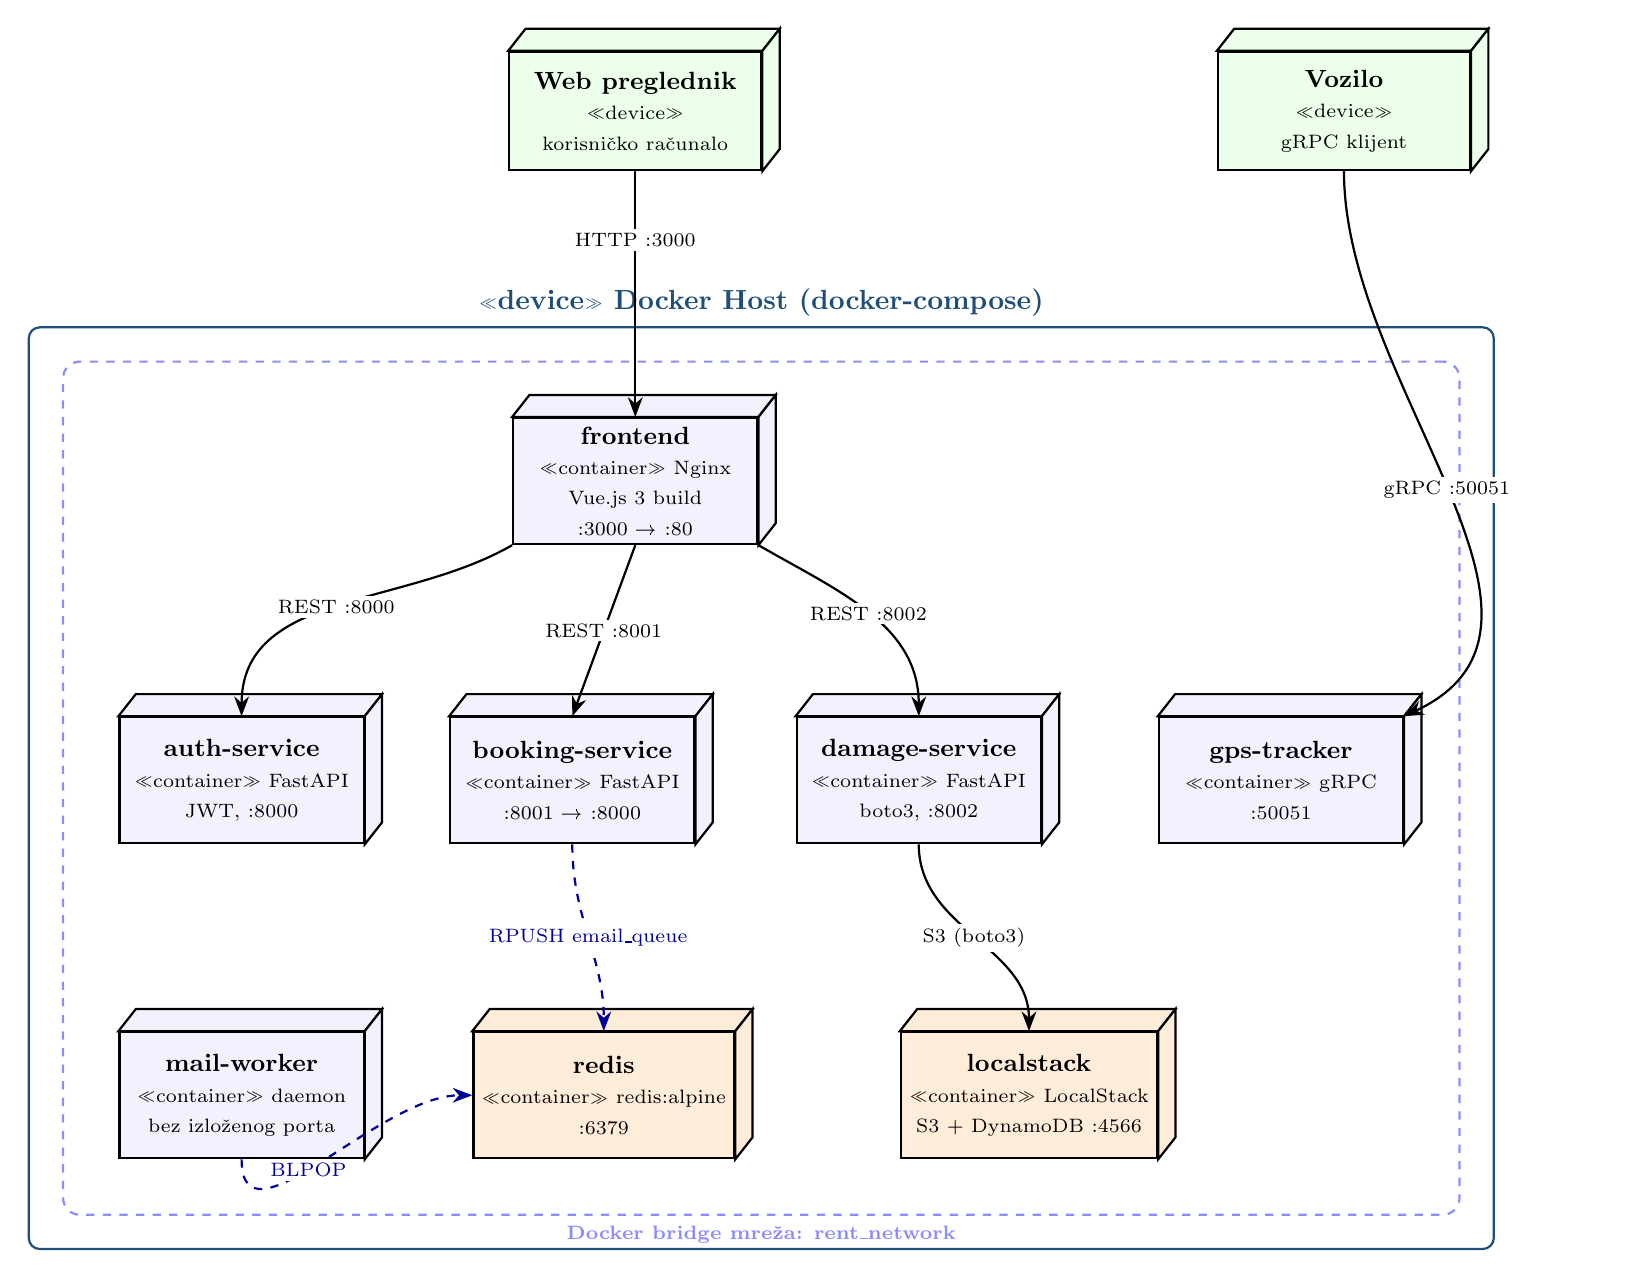
\begin{tikzpicture}[
  cont/.style={rectangle, draw, thick, fill=blue!5, minimum width=3.1cm, minimum height=1.6cm, align=center, font=\small, inner sep=3pt},
  infra/.style={rectangle, draw, thick, fill=orange!15, minimum width=3.1cm, minimum height=1.6cm, align=center, font=\small, inner sep=3pt},
  client/.style={rectangle, draw, thick, fill=green!8, minimum width=3.2cm, minimum height=1.5cm, align=center, font=\small, inner sep=3pt},
  link/.style={-{Stealth[length=2.5mm]}, thick},
  qlink/.style={-{Stealth[length=2.5mm]}, thick, dashed, blue!60!black},
  lbl/.style={font=\scriptsize, fill=white, inner sep=1.5pt}
]

% ===== External clients =====
\node[client] (browser) at (-2, 4.3) {\textbf{Web preglednik}\\{\scriptsize \guillemotleft device\guillemotright}\\{\scriptsize korisničko računalo}};
\node[client] (vehicle) at (7, 4.3) {\textbf{Vozilo}\\{\scriptsize \guillemotleft device\guillemotright}\\{\scriptsize gRPC klijent}};

% ===== Containers =====
\node[cont] (fe)   at (-2, -0.4) {\textbf{frontend}\\{\scriptsize \guillemotleft container\guillemotright{} Nginx}\\{\scriptsize Vue.js 3 build}\\{\scriptsize :3000 \textrightarrow{} :80}};
\node[cont] (auth) at (-7, -4.2) {\textbf{auth-service}\\{\scriptsize \guillemotleft container\guillemotright{} FastAPI}\\{\scriptsize JWT, :8000}};
\node[cont] (book) at (-2.8, -4.2) {\textbf{booking-service}\\{\scriptsize \guillemotleft container\guillemotright{} FastAPI}\\{\scriptsize :8001 \textrightarrow{} :8000}};
\node[cont] (dmg)  at (1.6, -4.2) {\textbf{damage-service}\\{\scriptsize \guillemotleft container\guillemotright{} FastAPI}\\{\scriptsize boto3, :8002}};
\node[cont] (gps)  at (6.2, -4.2) {\textbf{gps-tracker}\\{\scriptsize \guillemotleft container\guillemotright{} gRPC}\\{\scriptsize :50051}};
\node[cont] (mail) at (-7, -8.2) {\textbf{mail-worker}\\{\scriptsize \guillemotleft container\guillemotright{} daemon}\\{\scriptsize bez izloženog porta}};
\node[infra] (redis) at (-2.4, -8.2) {\textbf{redis}\\{\scriptsize \guillemotleft container\guillemotright{} redis:alpine}\\{\scriptsize :6379}};
\node[infra] (local) at (3, -8.2) {\textbf{localstack}\\{\scriptsize \guillemotleft container\guillemotright{} LocalStack}\\{\scriptsize S3 + DynamoDB :4566}};

% 3D deployment-node effect
\foreach \n in {fe,auth,book,dmg,gps,mail}{\deploybox{\n}{blue!5}}
\foreach \n in {redis,local}{\deploybox{\n}{orange!15}}
\foreach \n in {browser,vehicle}{\deploybox{\n}{green!8}}

% ===== Communication links =====
\draw[link] (browser.south) -- node[lbl, pos=0.28] {HTTP :3000} (fe.north);
\draw[link] (vehicle.south) to[out=-90, in=25] node[lbl, pos=0.5] {gRPC :50051} (gps.north east);
\draw[link] (fe.south west) to[out=-150, in=90] node[lbl, pos=0.5] {REST :8000} (auth.north);
\draw[link] (fe.south) -- node[lbl, pos=0.5] {REST :8001} (book.north);
\draw[link] (fe.south east) to[out=-30, in=90] node[lbl, pos=0.5] {REST :8002} (dmg.north);
\draw[qlink] (book.south) to[out=-90, in=90] node[lbl, pos=0.5] {RPUSH email\_queue} (redis.north);
\draw[qlink] (mail.south) to[out=-90, in=180] node[lbl, pos=0.45] {BLPOP} (redis.west);
\draw[link] (dmg.south) to[out=-90, in=90] node[lbl, pos=0.5] {S3 (boto3)} (local.north);

% ===== Network and host boundaries =====
\begin{scope}[on background layer]
\node[draw, dashed, thick, blue!45, rounded corners=6pt,
  fit=(fe)(auth)(book)(dmg)(gps)(mail)(redis)(local),
  inner sep=20pt,
  label={[blue!45, font=\bfseries\scriptsize]below:Docker bridge mreža: rent\_network}] (net) {};
\node[draw, thick, accent, rounded corners=4pt,
  fit=(net),
  inner sep=12pt,
  label={[accent, font=\bfseries]above:\guillemotleft device\guillemotright{} Docker Host (docker-compose)}] {};
\end{scope}

\end{tikzpicture}
}%
\caption{Dijagram raspodjele -- razvojno okruženje (Docker Compose + LocalStack)}
\label{fig:deploy-dev}
\end{figure}

Cijeli sustav izvodi se na jednom fizičkom čvoru, a izolacija servisa ostvaruje se kontejnerizacijom umjesto zasebnim strojevima. To je tipično za razvoj: jedna \texttt{docker-compose up} naredba podiže cjelokupnu topologiju. Tri REST veze (\texttt{:8000}, \texttt{:8001}, \texttt{:8002}) idu od frontenda prema aplikacijskim servisima, dvije isprekidane veze prikazuju asinkroni Redis red (\texttt{RPUSH}/\texttt{BLPOP}) između Booking-servisa i Mail-workera, a Damage-service piše fotografije u S3 koji simulira LocalStack. LocalStack na ovom čvoru zamjenjuje stvarne AWS servise -- razlika prema produkciji vidljiva je na sljedećem dijagramu.

% ========================================================================
\section{Dijagram raspodjele -- produkcijsko okruženje}

Dijagram na slici~\ref{fig:deploy-prod} prikazuje ciljnu (produkcijsku) raspodjelu sustava na AWS infrastrukturi. Ključna razlika u odnosu na razvojno okruženje jest da svaki infrastrukturni element koji LocalStack lokalno simulira ovdje postaje stvarni upravljani AWS servis: \texttt{localstack} se razlaže na \textbf{Amazon S3} (pohrana fotografija), \textbf{AWS Lambda} (obrada okinuta S3 eventom) i \textbf{Amazon DynamoDB} (perzistencija), Redis postaje \textbf{Amazon ElastiCache}, a aplikacijski kontejneri izvode se na \textbf{Amazon ECS / Fargate} klasteru iza \textbf{Amazon API Gateway-a}. Frontend se servira kao statički build iz S3 bucketa putem \textbf{CloudFront} CDN-a. Topologija veza ostaje identična -- mijenja se samo izvršno okruženje čvorova, što je izravna posljedica mikroservisne arhitekture.

\begin{figure}[H]
\centering
\resizebox{\textwidth}{!}{%
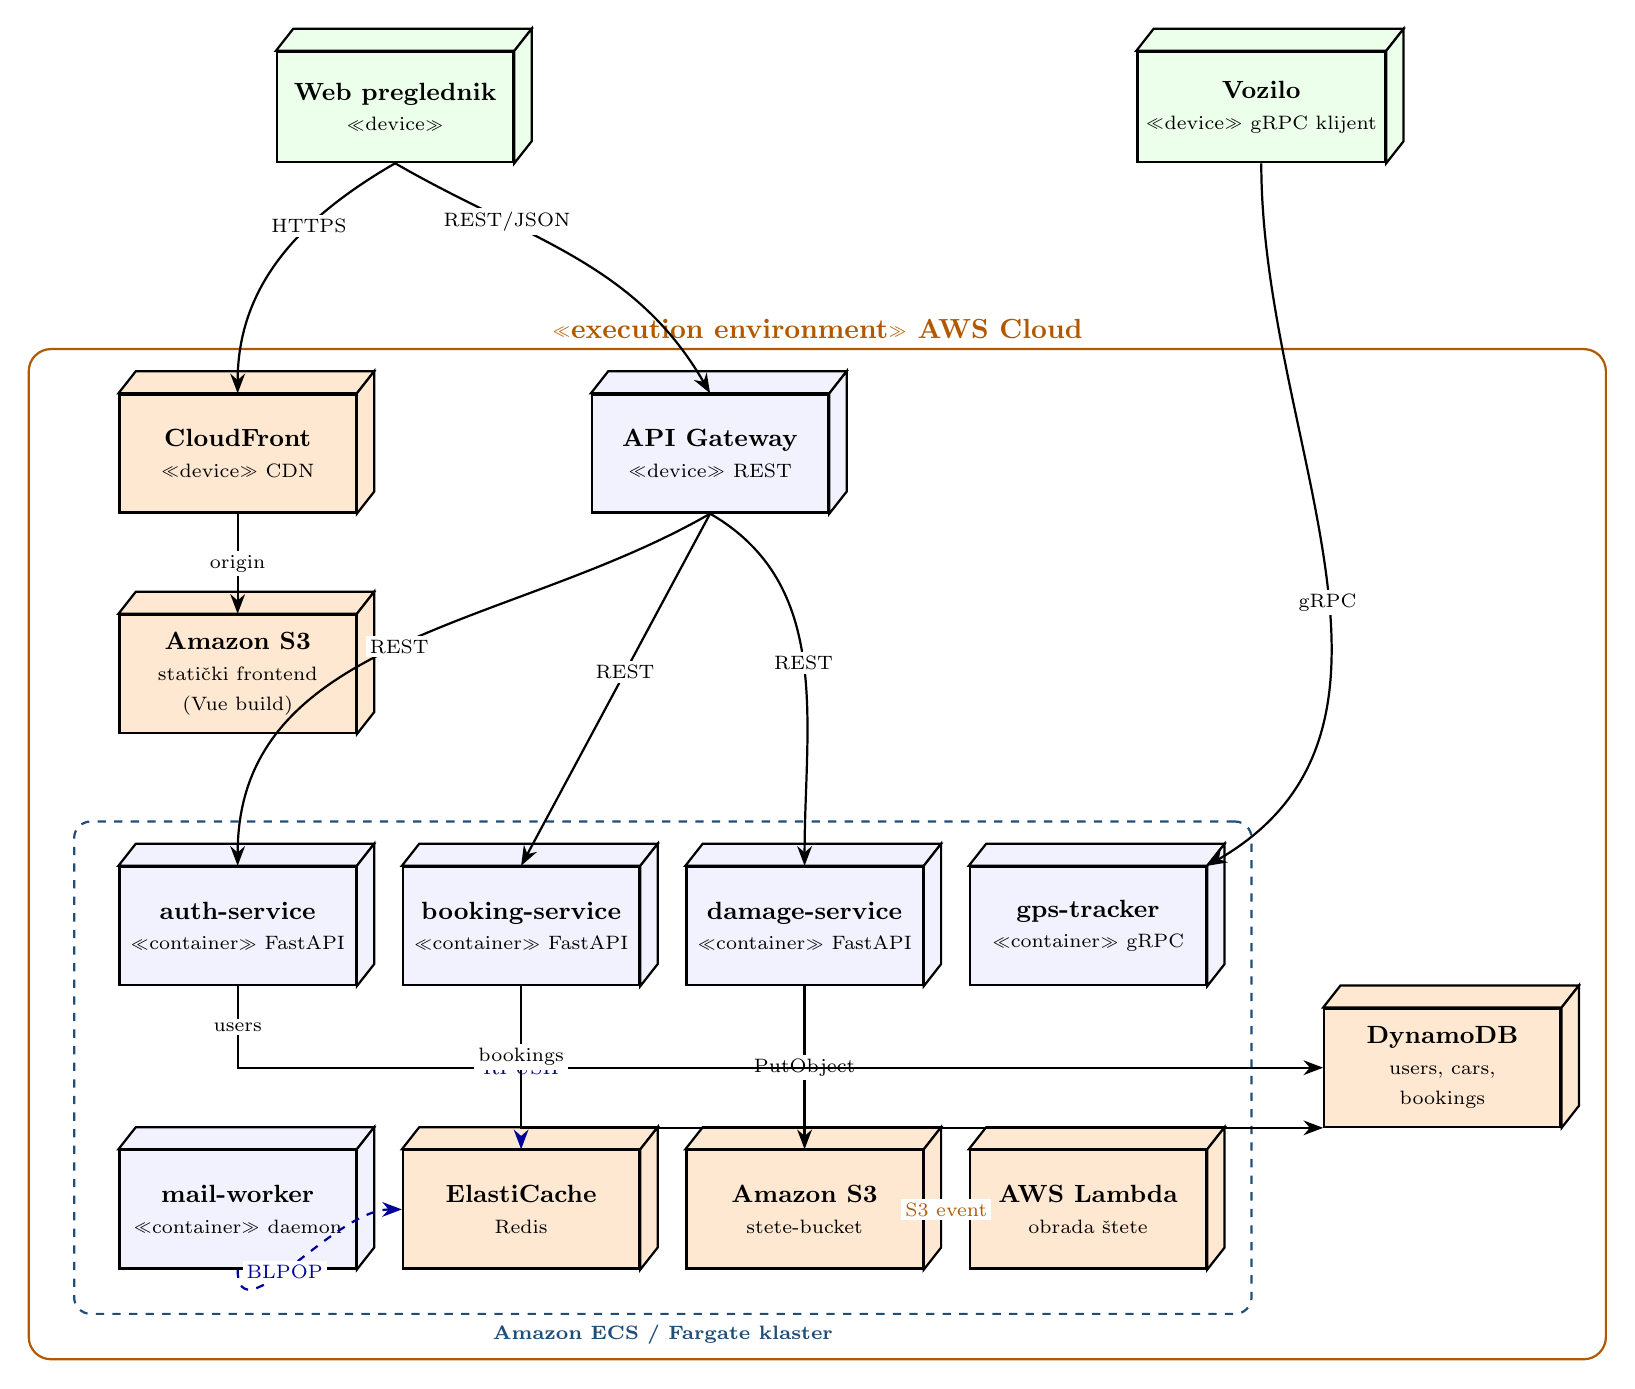
\begin{tikzpicture}[
  svc/.style={rectangle, draw, thick, fill=blue!5, minimum width=3.0cm, minimum height=1.5cm, align=center, font=\small, inner sep=3pt},
  aws/.style={rectangle, draw, thick, fill=orange!18, minimum width=3.0cm, minimum height=1.5cm, align=center, font=\small, inner sep=3pt},
  client/.style={rectangle, draw, thick, fill=green!8, minimum width=3.0cm, minimum height=1.4cm, align=center, font=\small, inner sep=3pt},
  link/.style={-{Stealth[length=2.5mm]}, thick},
  qlink/.style={-{Stealth[length=2.5mm]}, thick, dashed, blue!60!black},
  evlink/.style={-{Stealth[length=2.5mm]}, thick, dotted, orange!70!black},
  lbl/.style={font=\scriptsize, fill=white, inner sep=1.5pt}
]

% ===== External clients =====
\node[client] (browser) at (-4.5, 4.8) {\textbf{Web preglednik}\\{\scriptsize \guillemotleft device\guillemotright}};
\node[client] (vehicle) at (6.5, 4.8) {\textbf{Vozilo}\\{\scriptsize \guillemotleft device\guillemotright{} gRPC klijent}};

% ===== Edge / gateway =====
\node[aws] (cf)    at (-6.5, 0.4) {\textbf{CloudFront}\\{\scriptsize \guillemotleft device\guillemotright{} CDN}};
\node[aws] (s3web) at (-6.5, -2.4) {\textbf{Amazon S3}\\{\scriptsize statički frontend}\\{\scriptsize (Vue build)}};
\node[svc] (apigw) at (-0.5, 0.4) {\textbf{API Gateway}\\{\scriptsize \guillemotleft device\guillemotright{} REST}};

% ===== ECS cluster services =====
\node[svc] (auth) at (-6.5, -5.6) {\textbf{auth-service}\\{\scriptsize \guillemotleft container\guillemotright{} FastAPI}};
\node[svc] (book) at (-2.9, -5.6) {\textbf{booking-service}\\{\scriptsize \guillemotleft container\guillemotright{} FastAPI}};
\node[svc] (dmg)  at (0.7, -5.6) {\textbf{damage-service}\\{\scriptsize \guillemotleft container\guillemotright{} FastAPI}};
\node[svc] (gps)  at (4.3, -5.6) {\textbf{gps-tracker}\\{\scriptsize \guillemotleft container\guillemotright{} gRPC}};
\node[svc] (mail) at (-6.5, -9.2) {\textbf{mail-worker}\\{\scriptsize \guillemotleft container\guillemotright{} daemon}};

% ===== Managed data services =====
\node[aws] (redis)  at (-2.9, -9.2) {\textbf{ElastiCache}\\{\scriptsize Redis}};
\node[aws] (s3)     at (0.7, -9.2) {\textbf{Amazon S3}\\{\scriptsize stete-bucket}};
\node[aws] (lambda) at (4.3, -9.2) {\textbf{AWS Lambda}\\{\scriptsize obrada štete}};
\node[aws] (dynamo) at (8.8, -7.4) {\textbf{DynamoDB}\\{\scriptsize users, cars,}\\{\scriptsize bookings}};

% 3D deployment-node effect
\foreach \n in {auth,book,dmg,gps,mail,apigw}{\deploybox{\n}{blue!5}}
\foreach \n in {cf,s3web,redis,s3,lambda,dynamo}{\deploybox{\n}{orange!18}}
\foreach \n in {browser,vehicle}{\deploybox{\n}{green!8}}

% ===== Links =====
\draw[link] (browser.south) to[out=-150, in=90] node[lbl, pos=0.35] {HTTPS} (cf.north);
\draw[link] (cf.south) -- node[lbl, pos=0.5] {origin} (s3web.north);
\draw[link] (browser.south) to[out=-30, in=120] node[lbl, pos=0.3] {REST/JSON} (apigw.north);
\draw[link] (vehicle.south) to[out=-90, in=30] node[lbl, pos=0.55] {gRPC} (gps.north east);
\draw[link] (apigw.south) to[out=-150, in=90] node[lbl, pos=0.5] {REST} (auth.north);
\draw[link] (apigw.south) -- node[lbl, pos=0.45] {REST} (book.north);
\draw[link] (apigw.south) to[out=-30, in=90] node[lbl, pos=0.5] {REST} (dmg.north);
\draw[qlink] (book.south) to[out=-90, in=90] node[lbl, pos=0.5] {RPUSH} (redis.north);
\draw[qlink] (mail.south) to[out=-90, in=180] node[lbl, pos=0.45] {BLPOP} (redis.west);
\draw[link] (dmg.south) to[out=-90, in=90] node[lbl, pos=0.5] {PutObject} (s3.north);
\draw[evlink] (s3.east) -- node[lbl, pos=0.5] {S3 event} (lambda.west);
\draw[link] (auth.south) |- node[lbl, pos=0.25] {users} (dynamo.west);
\draw[link] (book.south) |- node[lbl, pos=0.25] {bookings} (dynamo.south west);

% ===== Cluster and cloud boundaries =====
\begin{scope}[on background layer]
\node[draw, dashed, thick, accent, rounded corners=6pt,
  fit=(auth)(book)(dmg)(gps)(mail),
  inner sep=16pt,
  label={[accent, font=\bfseries\scriptsize]below:Amazon ECS / Fargate klaster}] (ecs) {};
\node[draw, thick, orange!70!black, rounded corners=8pt,
  fit=(cf)(s3web)(apigw)(ecs)(redis)(s3)(lambda)(dynamo),
  inner sep=16pt,
  label={[orange!70!black, font=\bfseries]above:\guillemotleft execution environment\guillemotright{} AWS Cloud}] {};
\end{scope}

\end{tikzpicture}
}%
\caption{Dijagram raspodjele -- ciljno produkcijsko okruženje (AWS)}
\label{fig:deploy-prod}
\end{figure}

Usporedba dvaju dijagrama raspodjele izravno pokazuje vrijednost LocalStacka: razvojni i produkcijski dijagram dijele istu logičku topologiju, pa migracija na AWS ne zahtijeva preradu aplikacijskog koda nego samo zamjenu \texttt{endpoint\_url}-a i izvršnih čvorova. Točkasta veza \guillemotleft S3 event\guillemotright{} prikazuje obrazac koji u razvoju ostaje neaktivan (Lambda se ne okida), a u produkciji omogućuje automatsku obradu uploadanih fotografija šteta.

% ========================================================================
\section{Sekvencijski dijagram}

Slika~\ref{fig:sequence} prikazuje dva osnovna toka sustava. Prvi tok (koraci 1--4) ilustrira autentifikaciju: korisnik unosi kredencijale, Frontend ih prosljeđuje Auth-servisu koji vraća JWT token, a korisnik biva preusmjeren na Dashboard. Drugi tok (koraci 5--11) ilustrira kreiranje rezervacije s asinkronom obradom: Booking-service prima zahtjev, gura poruku u Redis red i odmah vraća potvrdu, dok Mail-worker neovisno preuzima poruku i šalje e-mail.

\begin{figure}[H]
\centering
\resizebox{\textwidth}{!}{%
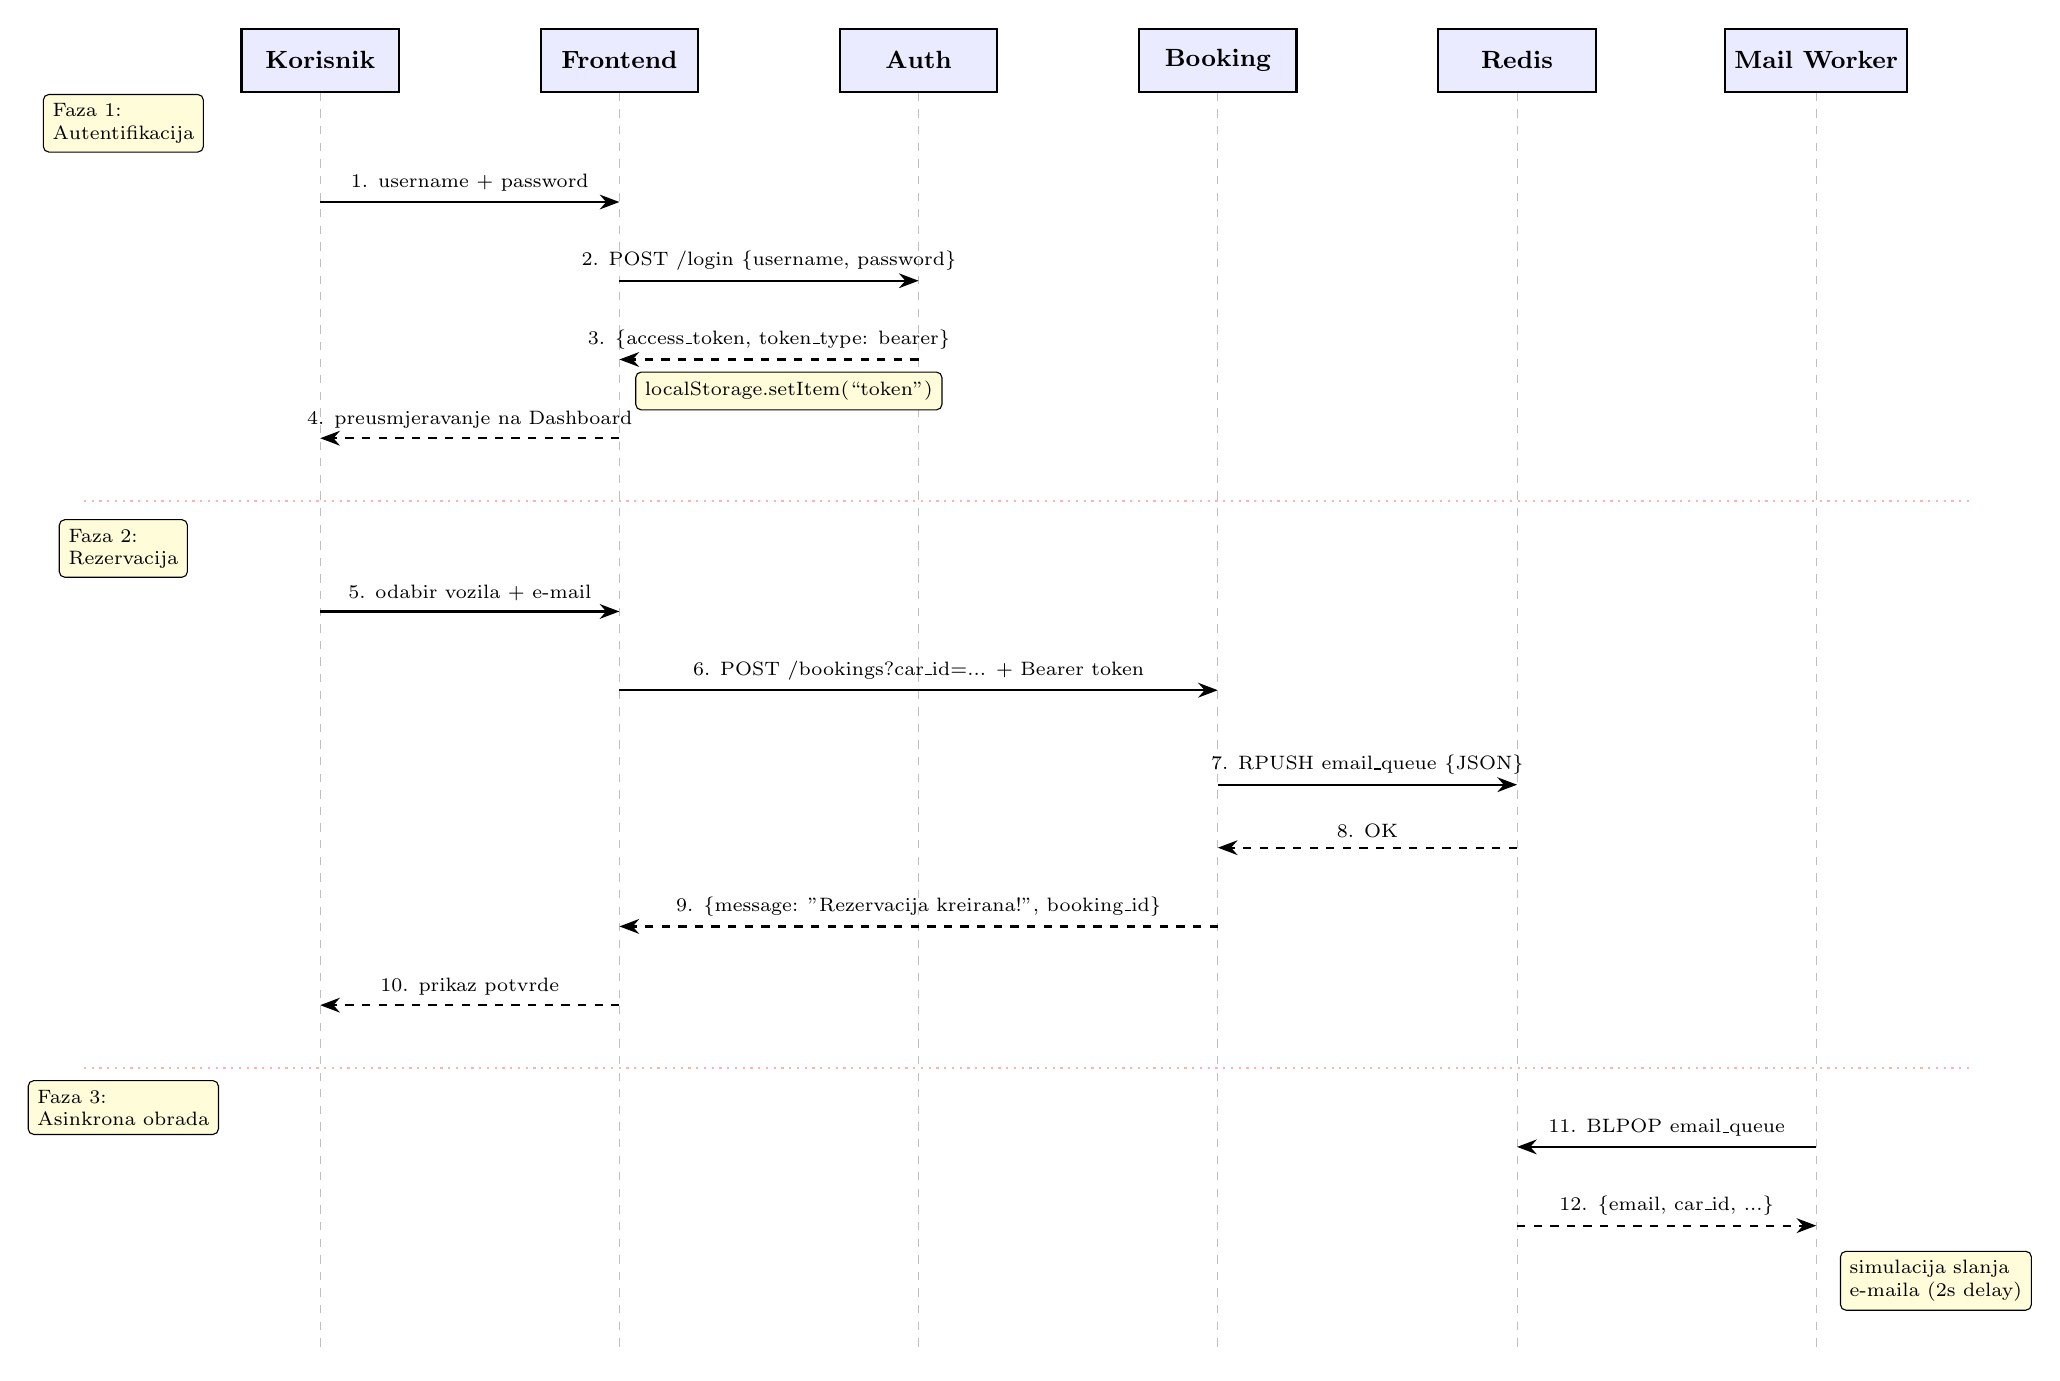
\begin{tikzpicture}[
  lifeline/.style={dashed, gray!50},
  msg/.style={-{Stealth[length=2.5mm]}, thick},
  ret/.style={-{Stealth[length=2.5mm]}, thick, dashed},
  box/.style={rectangle, draw, thick, fill=blue!8, minimum width=2cm, minimum height=0.8cm, font=\small\bfseries},
  note/.style={rectangle, draw, fill=yellow!15, font=\scriptsize, align=left, rounded corners=2pt}
]

% Actors
\node[box] (user) at (0,0) {Korisnik};
\node[box] (fe) at (3.8,0) {Frontend};
\node[box] (as) at (7.6,0) {Auth};
\node[box] (bs) at (11.4,0) {Booking};
\node[box] (rd) at (15.2,0) {Redis};
\node[box] (mw) at (19,0) {Mail Worker};

% Lifelines
\foreach \n in {user, fe, as, bs, rd, mw} {
  \draw[lifeline] (\n.south) -- ++(0,-16);
}

% ===== PHASE 1: Authentication =====
\node[note] at (-2.5, -0.8) {Faza 1:\\Autentifikacija};

\draw[msg] (0,-1.8) -- (3.8,-1.8) node[midway, above, font=\scriptsize] {1. username + password};
\draw[msg] (3.8,-2.8) -- (7.6,-2.8) node[midway, above, font=\scriptsize] {2. POST /login \{username, password\}};
\draw[ret] (7.6,-3.8) -- (3.8,-3.8) node[midway, above, font=\scriptsize] {3. \{access\_token, token\_type: bearer\}};
\draw[ret] (3.8,-4.8) -- (0,-4.8) node[midway, above, font=\scriptsize] {4. preusmjeravanje na Dashboard};

% Note: token stored
\node[note, right] at (4, -4.2) {\scriptsize localStorage.setItem(``token'')};

% Separator
\draw[thick, dotted, red!30] (-3,-5.6) -- (21,-5.6);

% ===== PHASE 2: Booking =====
\node[note] at (-2.5, -6.2) {Faza 2:\\Rezervacija};

\draw[msg] (0,-7) -- (3.8,-7) node[midway, above, font=\scriptsize] {5. odabir vozila + e-mail};
\draw[msg] (3.8,-8) -- (11.4,-8) node[midway, above, font=\scriptsize] {6. POST /bookings?car\_id=...  +  Bearer token};
\draw[msg] (11.4,-9.2) -- (15.2,-9.2) node[midway, above, font=\scriptsize] {7. RPUSH email\_queue \{JSON\}};
\draw[ret] (15.2,-10) -- (11.4,-10) node[midway, above, font=\scriptsize] {8. OK};
\draw[ret] (11.4,-11) -- (3.8,-11) node[midway, above, font=\scriptsize] {9. \{message: "Rezervacija kreirana!", booking\_id\}};
\draw[ret] (3.8,-12) -- (0,-12) node[midway, above, font=\scriptsize] {10. prikaz potvrde};

% Separator
\draw[thick, dotted, red!30] (-3,-12.8) -- (21,-12.8);

% ===== PHASE 3: Async mail =====
\node[note] at (-2.5, -13.3) {Faza 3:\\Asinkrona obrada};

\draw[msg] (19,-13.8) -- (15.2,-13.8) node[midway, above, font=\scriptsize] {11. BLPOP email\_queue};
\draw[ret] (15.2,-14.8) -- (19,-14.8) node[midway, above, font=\scriptsize] {12. \{email, car\_id, ...\}};

\node[note, right] at (19.3, -15.5) {\scriptsize simulacija slanja\\e-maila (2s delay)};

\end{tikzpicture}
}%
\caption{Sekvencijski dijagram -- autentifikacija, rezervacija i asinkrona obrada}
\label{fig:sequence}
\end{figure}

% ========================================================================
\section{Konceptualni model domene}

U ranoj fazi planiranja sustava izrađen je konceptualni dijagram koji prikazuje cjelovitu domenu rent-a-car poslovanja -- sve sudionike, funkcionalne blokove i baze podataka koje bi dovršeni sustav trebao obuhvatiti. Taj model je šire postavljen od trenutnog MVP-a i služi kao \emph{roadmap} za buduće iteracije; važno je jasno razlikovati što je implementirano u ovoj verziji, a što je zadržano kao prostor za daljnji razvoj.

\begin{figure}[H]
\centering
\IfFileExists{domena.png}{%
  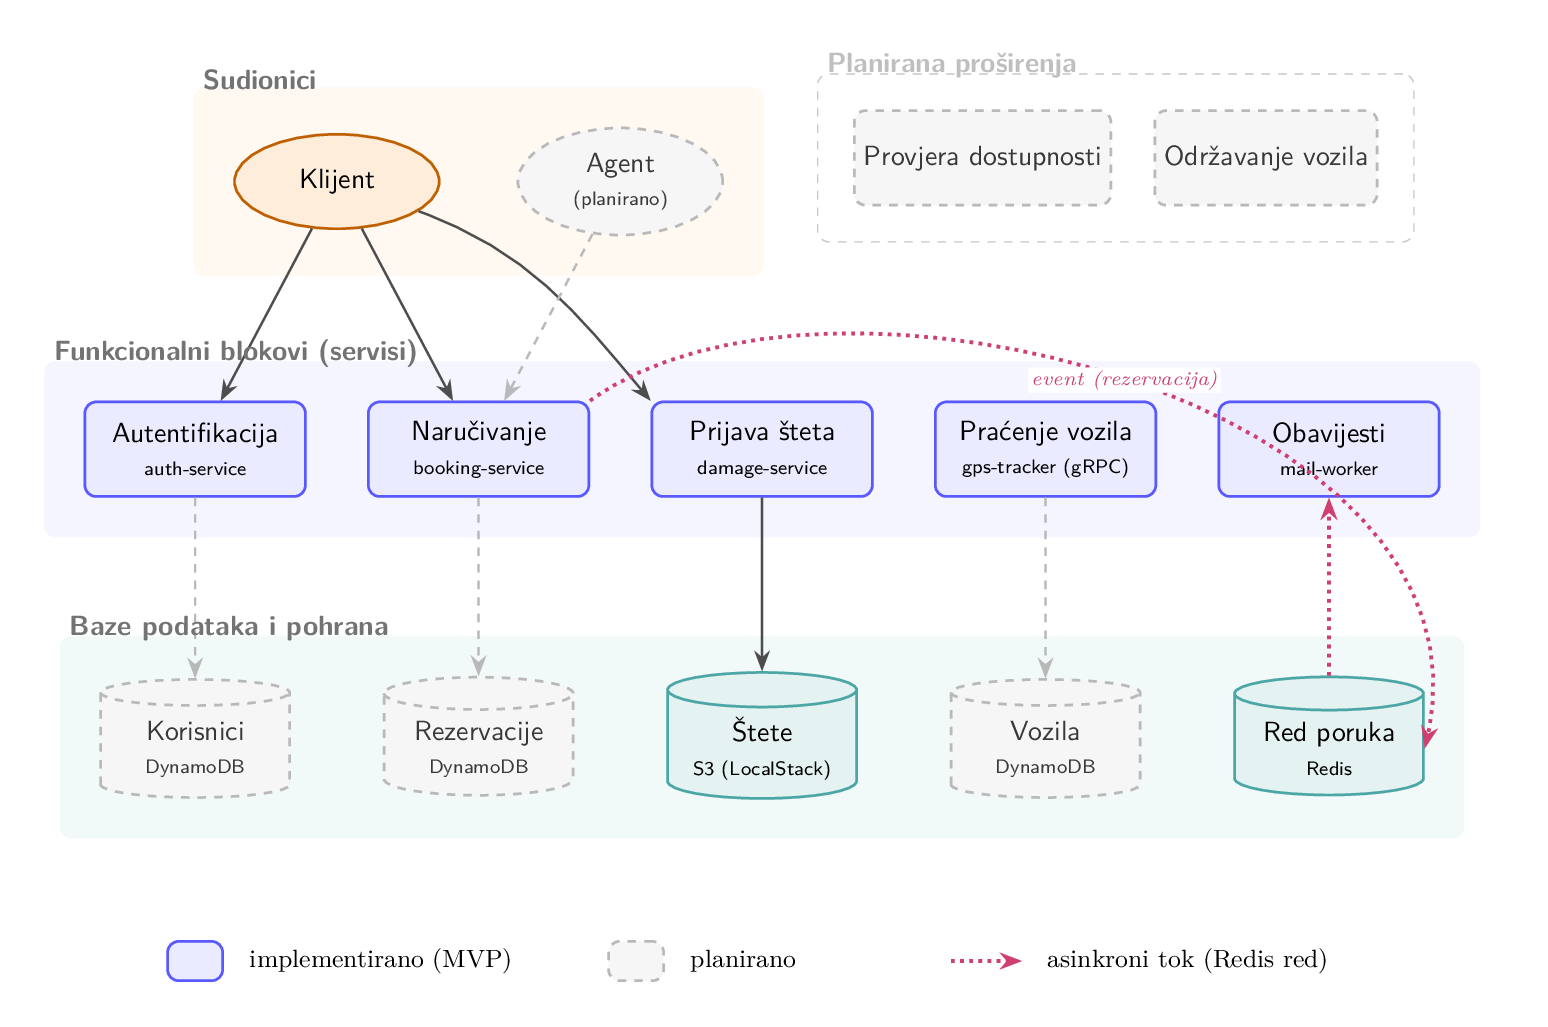
\includegraphics[width=\textwidth]{domena.png}%
}{%
  \fbox{\parbox[c][5cm][c]{0.8\textwidth}{\centering\itshape
    [Placeholder: spremi konceptualni dijagram kao\\
    \texttt{domena.png} u isti direktorij kao \texttt{dokumentacija.tex}]}}%
}
\caption{Konceptualni dijagram domene -- ciljno stanje sustava}
\label{fig:domena}
\end{figure}

Tablica~\ref{tab:pokrivenost} izravno mapira svaki element dijagrama na trenutni kod, označavajući što je dovršeno ($\checkmark$), a što je predviđeno za iduću iteraciju ($\times$).

\begin{table}[H]
\centering
\caption{Pokrivenost konceptualnog modela u MVP implementaciji}
\label{tab:pokrivenost}
\begin{tabularx}{\textwidth}{l c X}
\toprule
\textbf{Komponenta iz plana} & \textbf{MVP} & \textbf{Napomena} \\
\midrule
Autentifikacija korisnika      & $\checkmark$ & \texttt{auth-service}, JWT \\
Realtime praćenje vozila       & $\checkmark$ & \texttt{gps-tracker} preko gRPC-a \\
Naručivanje vozila (klijent)   & $\checkmark$ & \texttt{booking-service} \\
Frontend sučelje za klijente   & $\checkmark$ & Vue SPA (\texttt{Bookings}, \texttt{DamageUpload}) \\
Sustav za prijavu šteta        & $\checkmark$ & \texttt{damage-service} + S3 \\
Frontend za prijavu šteta      & $\checkmark$ & komponenta \texttt{DamageUpload.vue} \\
Sustav za slanje maila         & $\checkmark$ & \texttt{mail-worker} + Redis queue \\
\midrule
Baza korisnika                 & $\times$ & Kredencijali trenutno hardkodirani (\texttt{admin/admin}) \\
Baza vozila                    & $\times$ & Vozila su statička lista u \texttt{Bookings.vue} \\
Baza rezervacija               & $\times$ & Rezervacije prolaze kroz Redis queue bez perzistencije; DynamoDB u LocalStacku pripremljen za ovu namjenu \\
Održavanje vozila              & $\times$ & Domenski koncept, nije realiziran kao servis \\
Provjera dostupnosti vozila    & $\times$ & \texttt{booking-service} trenutno ne provjerava zauzetost termina \\
Frontend sučelje agenta        & $\times$ & Postoji samo jedinstveni frontend; agentski pogled predviđen uz uvođenje baze rezervacija \\
Poveznica šteta $\leftrightarrow$ rezervacija & $\times$ & \texttt{damage-service} uploada fotografiju bez referenciranja konkretne rezervacije \\
\bottomrule
\end{tabularx}
\end{table}

\subsection{Opseg MVP-a}

Fokus ove verzije je demonstracija \emph{komunikacijskih obrazaca} distribuiranog sustava -- REST, gRPC i asinkrona obrada putem message queue-a -- a ne potpuna poslovna logika rent-a-car operacije. Zbog toga su komponente koje zahtijevaju perzistentnu pohranu svjesno pojednostavljene: umjesto baza podataka korištene su hardkodirane vrijednosti i in-memory strukture, čime se zadržava jasnoća protoka poruka između servisa i izbjegava komplikacija vezana uz sheme, migracije i transakcije.

\subsection{Predviđena proširenja}

Prirodni sljedeći korak je uvođenje perzistencije. DynamoDB je već konfiguriran u LocalStacku, pa bi dodavanje tablica \texttt{users}, \texttt{cars} i \texttt{bookings} zahtijevalo samo ukidanje hardkodiranih vrijednosti u \texttt{auth-service}-u i \texttt{booking-service}-u te dodavanje čitanja i pisanja preko \texttt{boto3} klijenta. Nakon što \texttt{booking-service} dobije pristup bazi rezervacija, prirodno slijede: provjera dostupnosti termina, povezivanje uploadanih fotografija šteta s konkretnim rezervacijama te izrada zasebnog \emph{agentskog} sučelja koje bi dohvaćalo i ažuriralo te zapise. Održavanje vozila može se realizirati kao novi mikroservis s vlastitim schedulerom -- bez ikakvih izmjena u postojećim servisima, jedino dodavanjem novog čvora u Docker mrežu.

Ova postupnost ujedno demonstrira prednost mikroservisne arhitekture -- svaki od tih koraka može se implementirati neovisno, bez dodirivanja ostatka sustava.

% ========================================================================
\section{Zaključak}

Kroz ovaj projekt pokazao sam kako se jedan veći sustav može razbiti na neovisne servise koji međusobno komuniciraju putem mreže. Svaki servis ima jednu odgovornost i može se razvijati i deployati neovisno.

Korištenjem tri različita protokola -- REST, gRPC i Redis queue -- vidljivo je da nema jednog rješenja koje odgovara svim scenarijima. REST je jednostavan za CRUD i standardnu komunikaciju, gRPC ima smisla gdje je overhead JSON-a problematičan, a message queue rješava asinkronu obradu bez blokiranja.

Sustav se pokreće jednom naredbom i ne zahtijeva cloud infrastrukturu zahvaljujući LocalStacku. Sentry integracija pokrila je sve razine, od backenda do frontenda, što bi u produkcijskom okruženju bila osnova za dijagnostiku. Arhitektura je relativno lako proširiva -- novi servis dodaje se kao novi kontejner u mrežu, bez diranja postojećih.

\end{document}
